\begin{figure}
	\centering
	
	\begin{minipage}{0.435\linewidth}
		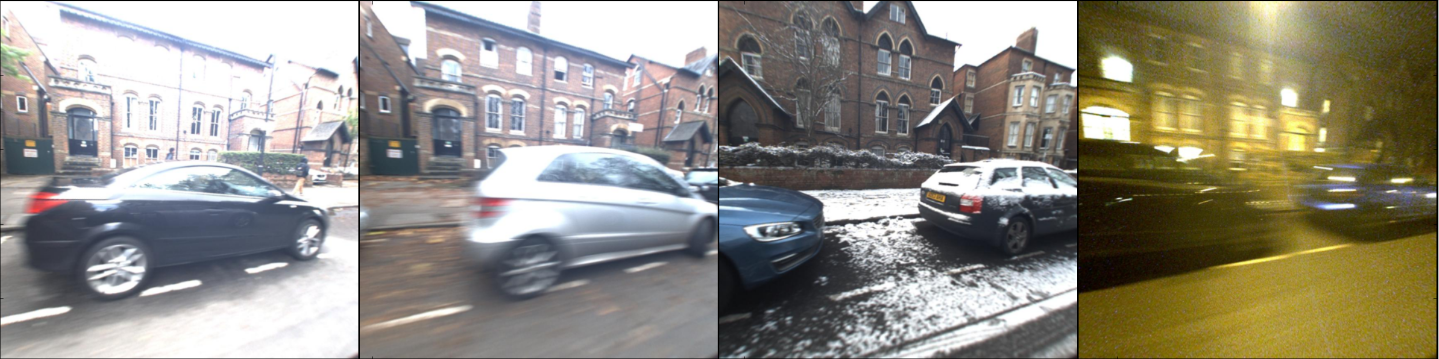
\includegraphics[width=\linewidth]{details/oxf_exs/ex1}
		
		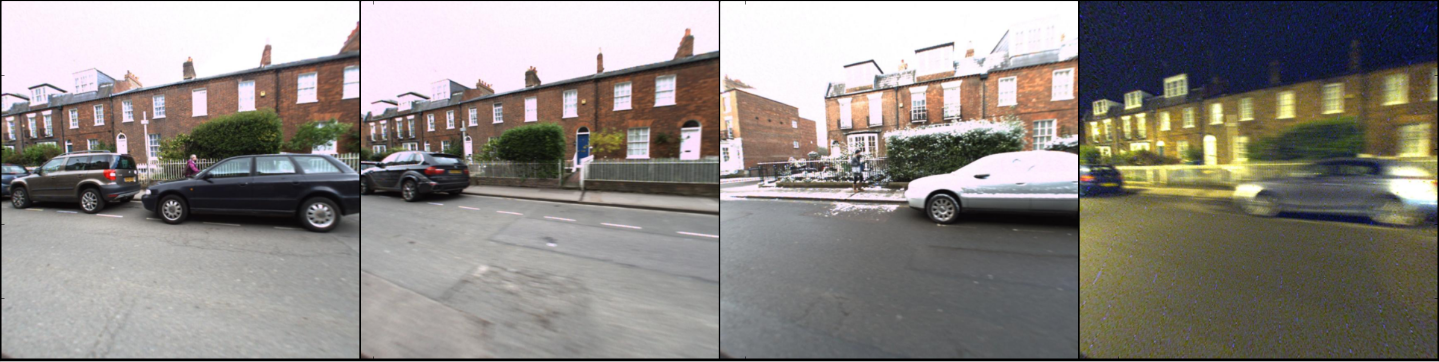
\includegraphics[width=\linewidth]{details/oxf_exs/ex2}
		
		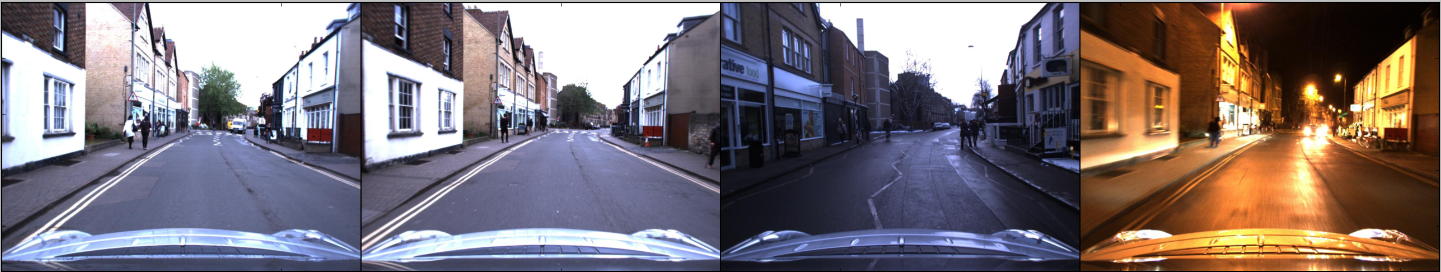
\includegraphics[width=\linewidth]{details/oxf_exs/ex4}
		
		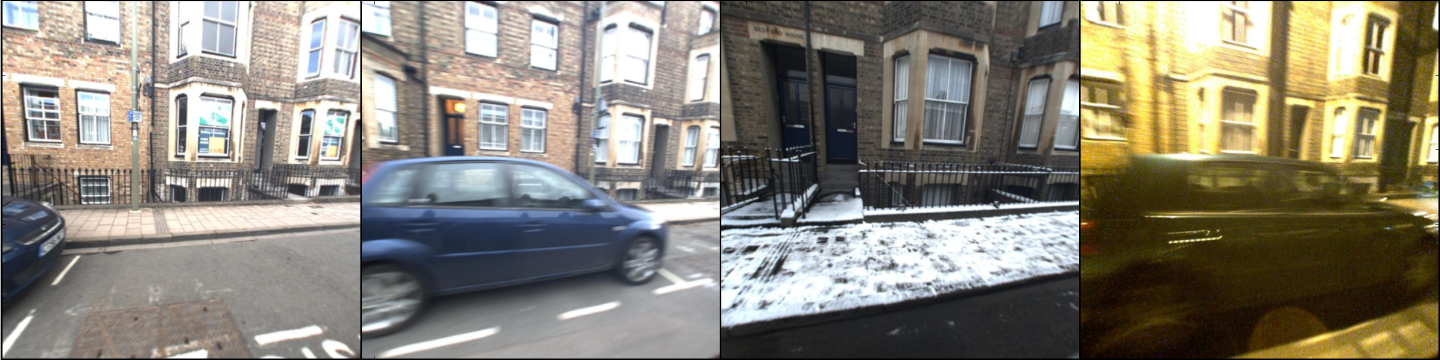
\includegraphics[width=\linewidth]{details/oxf_exs/ex6}
		
		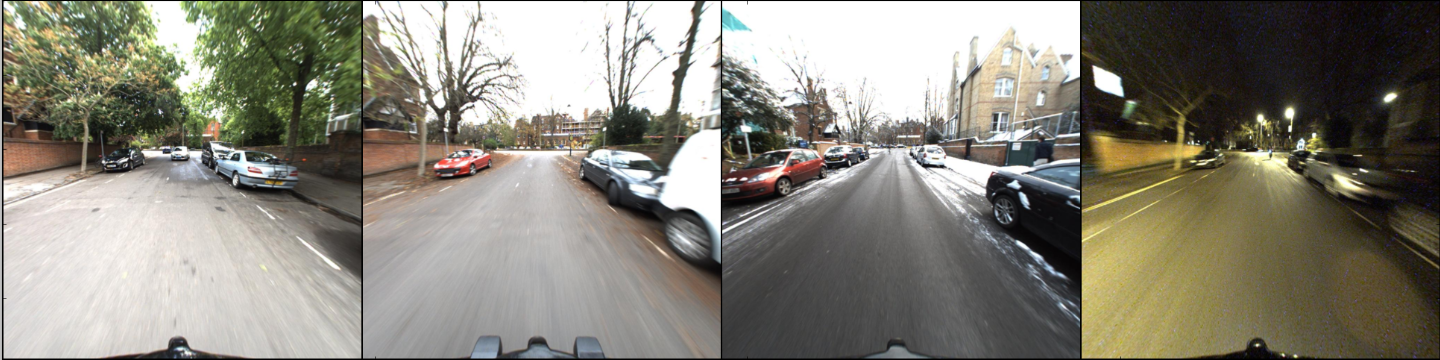
\includegraphics[width=\linewidth]{details/oxf_exs/ex3}
		
		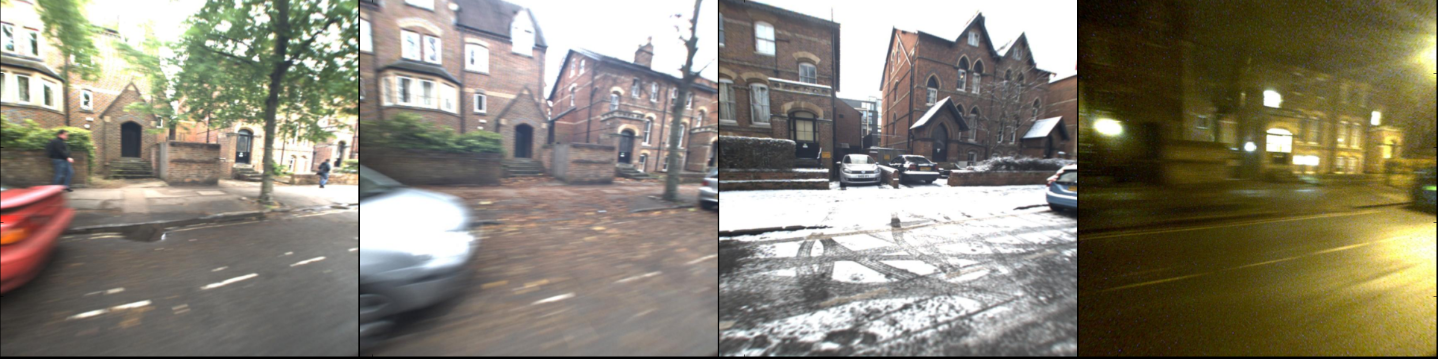
\includegraphics[width=\linewidth]{details/oxf_exs/ex5}
		
		\scriptsize
		\begin{tabularx}
		{\linewidth}{X X X X}
			Reference images & 	Long-term & Snow queries & Night queries
		\end{tabularx}
	\end{minipage}\hfill	
	\begin{minipage}{0.555\linewidth}
		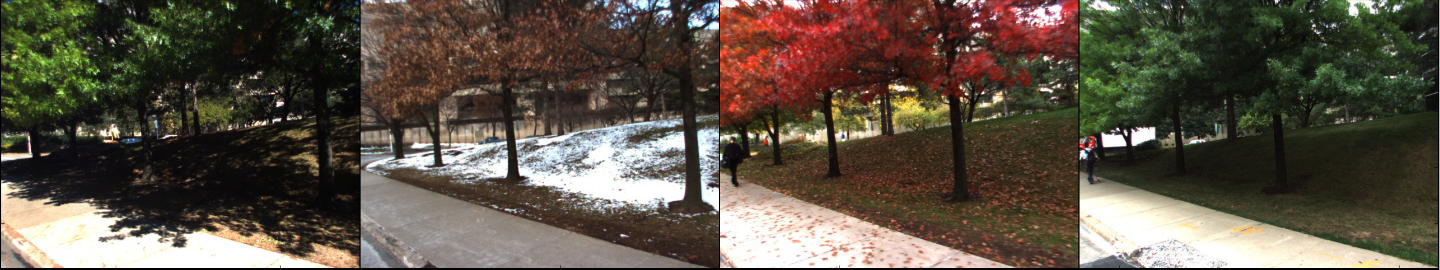
\includegraphics[width=\linewidth]{details/cmu_exs/ex1}
		
		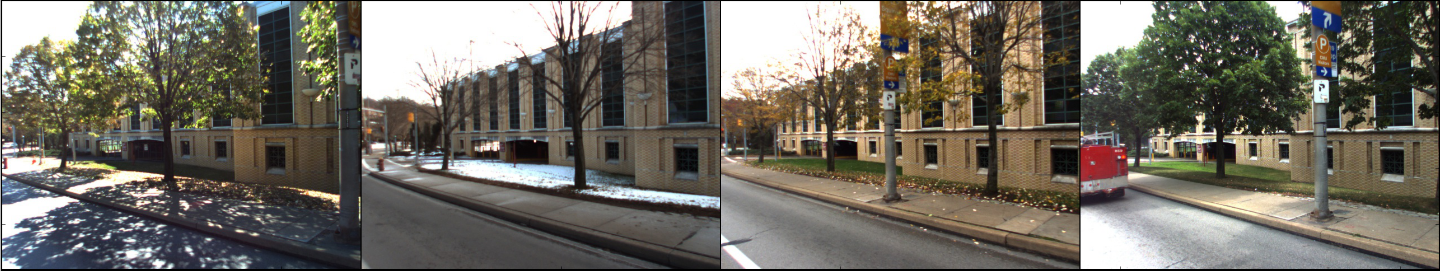
\includegraphics[width=\linewidth]{details/cmu_exs/ex6}
		
		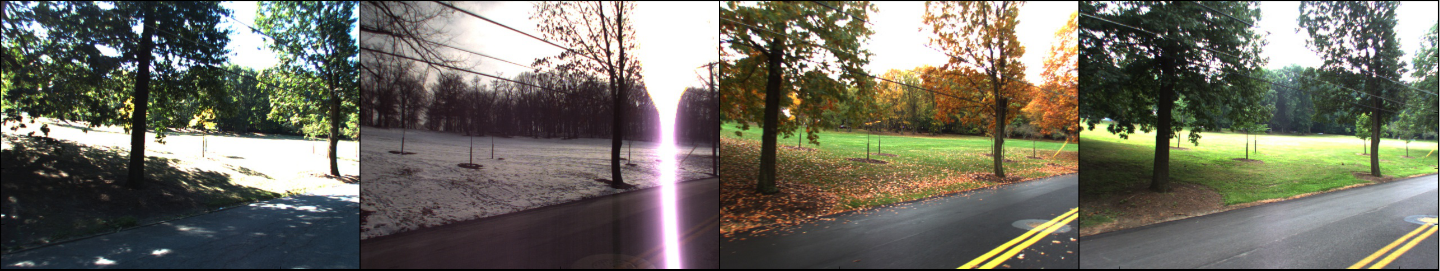
\includegraphics[width=\linewidth]{details/cmu_exs/ex4}	
		
		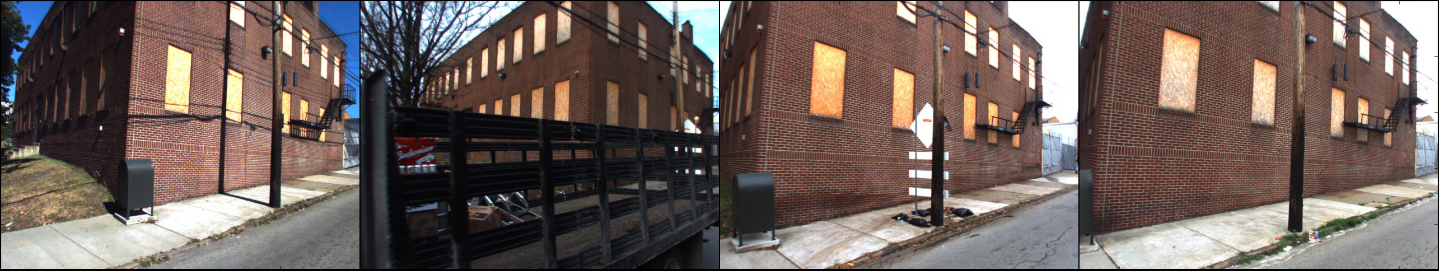
\includegraphics[width=\linewidth]{details/cmu_exs/ex2}	
		
		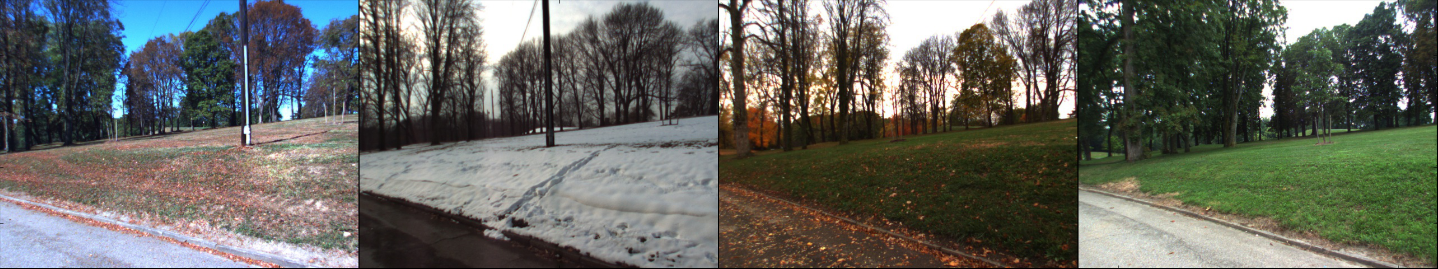
\includegraphics[width=\linewidth]{details/cmu_exs/ex3}	
		
		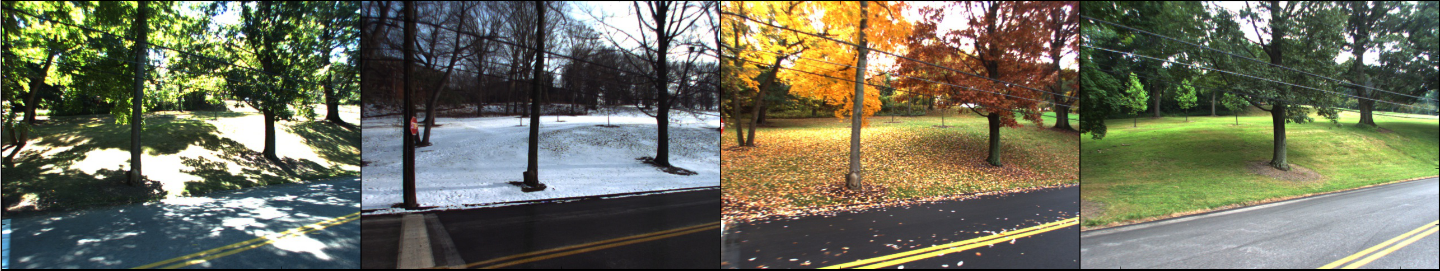
\includegraphics[width=\linewidth]{details/cmu_exs/ex5}	
		
		\scriptsize
		\begin{tabularx}{\linewidth}{X X X X}
			Reference images & Snow queries & Autumn queries & Long-term queries 
		\end{tabularx}
	\end{minipage}

	\caption[Examples of test images]{\label{fig:dataset} \textbf{Examples of test images :} we evaluate our proposal on 6 challenging localization sequences. Query image samples and the closest reference images in the database are presented from Oxford Robotcar~\cite{Maddern2016} (left) and CMU season dataset~\cite{Bansal2014a} (right).}
	
\end{figure}
